

\chapter{Dispersion}

\textit{Bestimmen sie die strahlende Rate, multi-exponentielle Zerfälle
}

% \section{Experiment}





%=============================================================
\section{2.5. Brechungsindex\protect\footnote{Parson, Kap. 3.1.5}\hfill w} 

\textit{Wie hängen Absorption und Dispersion eines Mediums zusammen?
Wie findet sich beides im Brechungsindex?}

Um den Brechungsindex eines Mediums zu bestimmen, nähert man die Elektronen als Lorentz-Oszillatoren mit Masse $m_{e}$, Dämpfung $\gamma$ und Federkonstante $k$. Die Elektronen werden vom externen elektrischen Feld $\vec{E}(t) = \vec{E}_{0} e^{i \omega t}$ zu Schwingungen angeregt und besitzen die Eigenfrequenz $\omega_{0} = \sqrt{k / m}$. Die Bewegungsgleichung für die Auslenkung $\vec{x}(t)$ aus der Ruhelage lautet dann

\begin{equation}
    m_{e} \frac{d^{2}\vec{x}(t)}{dt^{2}} + \gamma \frac{d\vec{x}(t)}{dt} + k \vec{x}(t) = e \left( \vec{E}(t) + \frac{\vec{P}(t)}{3\varepsilon_{0}} \right) \quad .
\end{equation}

Da die Reaktion des Materials auf das elektrische Feld berücksichtigt werden muss, befindet sich auf der rechten Seite der Ausdruck für das \emph{lokale} elektrische Feld am Ort der Elektronen. Dies enthält die Polarisation $\vec{P}(t) = \vec{x}(t) e n$ mit der Teilchendichte $n$. Der Faktor $1/3$ folgt aus der zufälligen Orientierung der Moleküle in Flüssigkeiten und des dadurch nötigen Mittelungsprozesses.

Durch Lösen der Differentialgleichung lässt sich dann die frequenzabhängige Suszeptibilität $\chi(\omega) = P(t) / \varepsilon_{0} E(t)$ bestimmen:

\begin{equation}
    \chi(\omega) = \frac{n e^{2}}{\varepsilon_{0} m_{e}} \frac{1}{\omega_{0}^{2} - \frac{n e^{2}}{3 \varepsilon_{0} m_{e}} - \omega^{2} + i \gamma \omega}
\end{equation}

Falls die Moleküle Elektronen mit verschiedenen Eigenfrequenzen enthalten, so ist die Suszeptibilität die mit der Oszillatorstärke gewichtete Summe der Einzelsuszeptibilitäten.

Gemäß $\varepsilon = 1 + \chi$ folgt dann der komplexe Brechungsindex $\tilde{n}(\omega) = \sqrt{\varepsilon(\omega)} = n - i \kappa$. Betrachtet man nun eine ebene Welle mit Wellenvektor $k = \tilde{n}\omega/c$, so wird direkt die Bedeutung des Real- und Imaginäteils des Brechungsindex klar:

\begin{equation}
    E \sim e^{i(kx - \omega t)} = e^{i(\frac{\omega}{c}x (n-i\kappa) - \omega t)} = e^{i(\frac{\omega}{c}n x - \omega t)} \cdot e^{- \frac{\omega}{c} \kappa x}
\end{equation}

$\kappa$ bestimmt demnach die Abklingkonstante der Welle, d.h.\ der Imaginärteil des Brechungsindex verursacht Absorption. Der Realteil hingegen legt die (frequenzabhängige) Ausbreitungsgeschwindigkeit der Welle fest und beschreibt somit die Dispersion im Material. Für Frequenzen entfernt von der Resonanzfrequenz $\omega_{0}$ nimmt $n$ mit der Frequenz zu (normale Dispersion). In der Nähe von $\omega_{0}$ kehrt sich dieses Verhalten um und $n$ sinkt mit steigender Frequenz (anormale Dispersion).

\begin{figure}[htb]
    \centering
    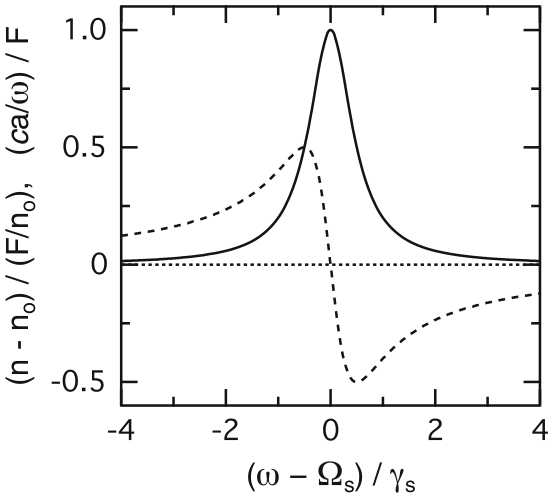
\includegraphics[width = 0.5 \textwidth]{Dispersion_Absorption.png}
    \caption{Absorption (durchgezogene Linie) und Dispersion (gestrichelte Linie) als Funktion der Frequenz nach dem Oszillatormodell.}
    % Aus Parson, S. 100
\end{figure}

%=============================================================
\section{2.6. Local field correction\protect\footnote{Parson, Kap. 3.1.6}\hfill *} 

\textit{Dies wird wohl neu für sie sein: Welches Feld erfährt ein
Molekül, das in einem Medium eingeschlossen ist?  Was
unterscheidet die verschiedenen Methoden der Korrektur?}

Bisher wurde die makroskopische Polarisierung zur Bestimmung des elektrischen Feldes $\vec{E}_{med}$ in einem Medium herangezogen. Ist nun ein Molekül in dem Medium eingeschlossen, wechselwirkt es mit dem Medium und spürt so effektiv eine veränderte lokale Feldstärke $\vec{E}_{loc}$.

In einem einfachen Modell ist das Molekül eingebettet in einem sphärischen Hohlraum. Das elektrische Feld im Medium führt zu einer Oberflächenladung am Hohlraum, sodass das Molekül ein lokales elektrisches Feld
\begin{equation}
    \vec{E}_{cav} = \left(\frac{3n^{2}}{2n^{2}+1}\right) \vec{E}_{med}
\end{equation}
spürt. Dies ist abhängig vom Brechungsindex des Materials.

Durch das Feld im Hohlraum wird das Molekül polarisiert und generiert so ein Reaktionsfeld, welches auf das elektrische Feld im Medium zurückwirkt. Das obige Modell muss deshalb um die sogenannte Lorentz-Korrektur erweitert werden, sodass sich ein lokales Feld
\begin{equation}
    \vec{E}_{L} = \left(\frac{n^{2}+2}{3}\right) \vec{E}_{med}
\end{equation}
ergibt.



\printbibliography[segment=\therefsegment,heading=subbibliography]
